\chapter{Zabezpieczenie bazy danych}
	\section{System GRANT}
	Podstawową formą zabezpieczenia in-dbase w psql jest system GRANT/REVOKE. Sprowadza się do bardzo prostych zapytań:
	\begin{lstlisting}
	GRANT uprawnienie ON objekt TO rola;
	REVOKE uprawnienie ON objekt TO rola;
	\end{lstlisting}
Dostępna lista uprawnień to:
\begin{itemize}
	\item SELECT
	
Pozwala na wykonanie operacji SELECT z obiektów tabeli. Jest to podstawowe uprawnienie konieczne dla dostępu do tabeli.
	\item INSERT
	
Pozwala na tworzenie nowych wierszy. Można wskazać również konkretne kolumny dla których uprawnienie będzie dostępne. Uprawnia również do COPY FROM.
	\item UPDATE
	
Pozwala na aktualizację istniejącego wiersza
	
	\item DELETE
	
Pozwala usunąć pojedyńczy wiersz
	\item TRUNCATE
	
Czyści zawartość tabeli, pozostawia strukturę.
	\item REFERENCES
Pozwala na tworzenie kluczy i indeksów.

	\item TRIGGER
	
Uprawnia do tworzenia wyzwalaczy
	\item CREATE
	
Dla bazy pozwala na tworzenie schematów, w schematach tabel, w przypadku tabel również indeksów, oraz obiektów tymczasowych
o to create, alter, or drop his own user's user mappings associated with that server.
	
\end{itemize}	
	\section{Row-level security}
	Szczególną formą systemu GRANT jest tzw. Row-level Security (RLS), istniejące w Postgresql od wersji 9.5.
	\begin{lstlisting}
	CREATE TABLE hydranty (  
	user_role_name NAME,
	typ TEXT,
	srednica TEXT
	);
	
	ALTER TABLE hydranty ENABLE ROW LEVEL SECURITY;
	
	CREATE POLICY uzytkownik_hydrant ON hydranty  
	FOR SELECT, DELETE
	USING(user_role_name = current_user);
	
	CREATE POLICY uzytkownik_hydrant ON hydranty  
	FOR SELECT, DELETE
	WITH CHECK(user_role_name = current_user);
	\end{lstlisting}
	
	\section{Kopia bezpieczeństwa}
	\subsection{pg\_dump}
	
	Podstawową formą tworzenia kopii bezpieczeństwa jest polecenie pg\_dump. Wywołujemy je ze wskazaniem bazy danych, tabel, oraz formatu kopii. 
	
	Przykładowe wywołanie poniżej:
	\begin{lstlisting}
pg_dump baza \> plik.sql
\end{lstlisting}

Jest to najprostsza forma, wykonująca kopię bezpieczeństwa całości wskazanej bazy danych (wszystkie schematy, oraz funkcje). Istotnym jest zaznaczenie że operator wykonujący polecenie pg\_dump, musi posiadać uprawnienia dostępu do wszystkich obiektów w wskazanej bazie. A więc najczęściej operację tą wykonywać będzie superużytkownik bazy danych.

Kolejny przykład to replikacja jednorazowa pomiędzy dwoma serwerami bazy danych.
	
\begin{lstlisting}
pg_dump -h localhost baza | psql -h 192.168.0.100 baza1
\end{lstlisting}
	
Inne ważne ustawienia pg\_dump to:
\begin{itemize}
\item -E encoding
\item -F format
\item -n schema / -N schema
\item -t schema / -T schema
\item -d dbname -h host -p port -U username
\end{itemize}

W przypadku przełącznika format możemy przyjąć następujące wartości:
\begin{itemize}
	\item p plain
	\item c custom
	\item d directory
	\item t tar
\end{itemize} 
Standardowo powinniśmy używać formatu plain jeśli mamy zamiar korzystać z przywracania przy pomocy \textbf{psql} lub \textbf{pgAdmin}, lub custom/directory dla przywracania przy pomocy \textbf{pg\_restore}

Dla zarchiwizowania bazy danych znajdującej się na odległym serwerze do kopii bezpieczeństwa użyjemy np. takiego polecenia:

\colorbox{code-gray}{pg\_dump -h 192.168.0.102 -U osm -d osm -Fc -f osm.sql}

\noindent Przywrócenia takiej bazy zostanie analogicznie wykonane poleceniem: 

\colorbox{code-gray}{pg\_restore -h 192.168.0.102 -U osm -d osm -f osm.sql}
	\subsection{pgAdmin}
	W przypadku pgAdmin'a wykonywanie kopii bezpieczeństwa dokonuje się dla każdego poziomu (baza, schema, tabela) w podobny sposób. Opcja ta dostępna jest między innymi z menu kontekstowego (prawy klawisz myszy). 
		\begin{figure}[!ht]
			\centering
			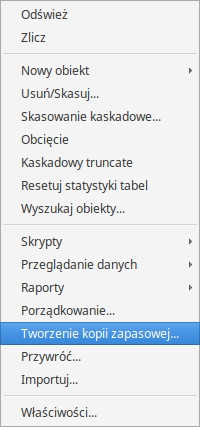
\includegraphics[width=4cm]{pgadmin_wykonanie_kopii}
			\caption{Menu kontekstowe pgAdmin}
		\end{figure}
	Następnie w oknie wskazujemy plik docelowy na dysku, tryb wykonania kopii (zwykły, użytkownika, katalog lub TAR), kodowanie znaków, oraz rolę użytkownika (preferowana ta sama rola, która jest właścicielem tabeli).	
		\begin{figure}[!ht]
			\centering
			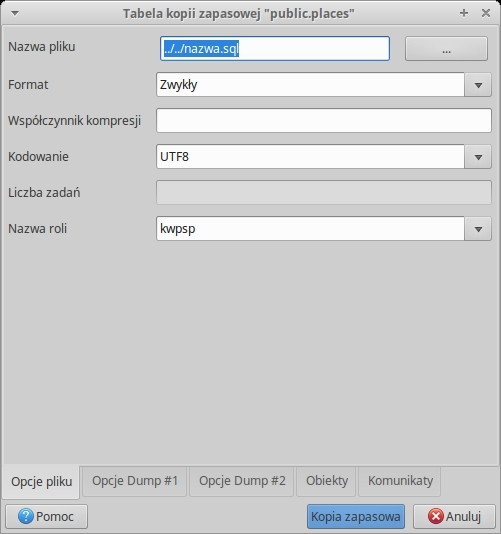
\includegraphics[width=5cm]{pgadmin_ustawienia_kopii}
			\caption{pgAdmin - ustawienia kopii zapasowej}
		\end{figure}
	Należy pamiętać że w przypadku przywracania tabeli z kopii, z poziomu programu pgAdmin, konieczne jest użycie wstawień wierszy, dostępne z drugiej zakładki. 
	\begin{figure}[!ht]
		\centering
		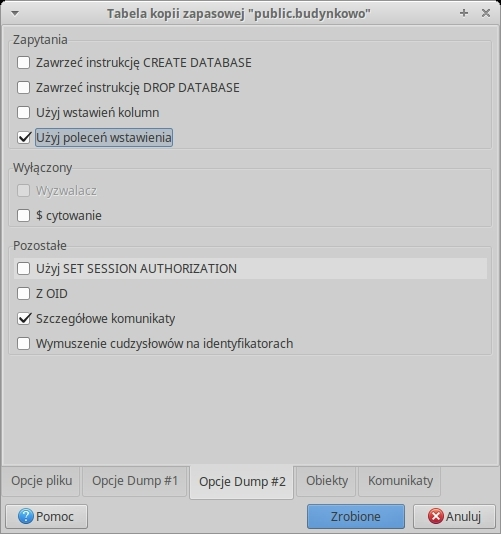
\includegraphics[width=5cm]{pgadmin_insert}
		\caption{Kopia zapasowa - Użyj wstawień wierszy}
		\end{figure}
	
	
%	\subsection{Punkty przywracania}
